\documentclass[../main.tex]{subfiles}
\graphicspath{{\subfix{../images/}}}


\begin{document}

\subsection{Úkol 3 - Příklad 11}
\subsubsection{Zadání}


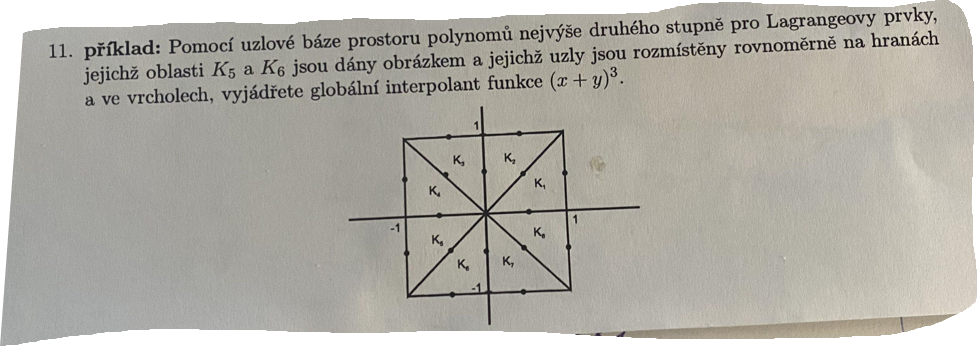
\includegraphics[width=1\textwidth]{images/zadani-ukol3-pr11.png}



\subsubsection{Řešení}
Označme $f(x,y) = (x+y)^3$.


Nejprve najděme lokální interpolant pro $K_6$.

Začněme nalezením uzlové báze. Máme následující:

\begin{itemize}
    \item $N_1(f) = f (0,0) = 0 $
    \item $N_2(f) = f (0,-1/2) = -1/8$
    \item $N_3(f) = f (0,-1) = -1$
    \item $N_4(f) = f (-1/2,-1) = -27/8$
    \item $N_5(f) = f (-1,-1) = -8$
    \item $N_6(f) = f (-1/2,-1/2) = -1$
\end{itemize}

Hledáme bázi:\begin{equation}\label{eq:bazeukol}
    \Phi_j(x,y) = a_j +b_jx +c_jx +d_jx^2+e_jy^2+f_jxy
\end{equation}

a vyžadujeme podmínku $N_j(I_l)=\delta_{jl}$

Z toho dostáváme následující soustavy rovnic $\forall j \in \hat{6}$

\begin{align*}
    a_j &= \delta_{1j}\\
    a_j - \frac{1}{2}c_j + \frac{1}{4}e_j &= \delta_{2j}\\
    a_j -c_j +e_j &= \delta_{3j}\\
    a_j -\frac{1}{2}b_j -c_j +\frac{1}{4}d_j +e_j +\frac{1}{2} &= \delta_{4j}\\
    a_j -b_j-c_j+d_j+e_j+f_j &= \delta_{5j}\\
    a_j -\frac{1}{2}b_j -\frac{1}{2}c_j +\frac{1}{4}d_j + \frac{1}{4}e_j + \frac{1}{4}f_j&= \delta_{6j}\\
\end{align*}


Tuto soustavu můžeme úsporněji napsat jako:

\hfuzz=20pt
\begin{gather*}
    \left(\begin{matrix}
        1 & 0 & 0 & 0 & 0 & 0 \\
        1 & 0 & -\frac{1}{2} & 0 & \frac{1}{4} & 0 \\
        1 & 0 & -1 & 0 & 1 & 0 \\
        1 & -\frac{1}{2} & -1 & \frac{1}{4} & 1 & \frac{1}{2} \\
        1 & -1 & -1 & 1 & 1 & 1 \\
        1 & -\frac{1}{2} & \frac{-1}{2} & \frac{1}{4} & \frac{1}{4} & \frac{1}{4}
        \end{matrix}\right)
        \left(\begin{matrix}
            a_1 & a_2 & a_3 & a_4 & a_5 & a_6 \\
            b_1 & b_2 & b_3 & b_4 & b_5 & b_6 \\
            c_1 & c_2 & c_3 & c_4 & c_5 & c_6 \\
            d_1 & d_2 & d_3 & d_4 & d_5 & d_6 \\
            e_1 & e_2 & e_3 & e_4 & e_5 & e_6 \\
            f_1 & f_2 & f_3 & f_4 & f_5 & f_6 
            \end{matrix}\right)
        =
        \left(\begin{matrix}
            1 & 0 & 0 & 0 & 0 & 0 \\
            0 & 1 & 0 & 0 & 0 & 0 \\
            0 & 0 & 1 & 0 & 0 & 0 \\
            0 & 0 & 0 & 1 & 0 & 0 \\
            0 & 0 & 0 & 0 & 1 & 0 \\
            0 & 0 & 0 & 0 & 0 & 1
            \end{matrix}\right)
\end{gather*}
\hfuzz=0pt

Po vyřešení dostaneme: 

\begin{gather*}
        \left(\begin{matrix}
            a_1 & a_2 & a_3 & a_4 & a_5 & a_6 \\
            b_1 & b_2 & b_3 & b_4 & b_5 & b_6 \\
            c_1 & c_2 & c_3 & c_4 & c_5 & c_6 \\
            d_1 & d_2 & d_3 & d_4 & d_5 & d_6 \\
            e_1 & e_2 & e_3 & e_4 & e_5 & e_6 \\
            f_1 & f_2 & f_3 & f_4 & f_5 & f_6 
            \end{matrix}\right)
        =
        \left(\begin{matrix}
            1 & 0 & 0 & 0 & 0 & 0 \\
            0 & 4 & -1 & 0 & 1 & -4 \\
            3 & -4 & 1 & 0 & 0 & 0 \\
            0 & 0 & 2 & -4 & 2 & 0 \\
            2 & -4 & 2 & 0 & 0 & 0 \\
            0 & 4 & -4 & 4 & 0 & -4
            \end{matrix}\right)
\end{gather*}


Tedy dostaneme následující uzlové funkce: 

\begin{itemize}
    \item $\Phi_1(x,y) = 1 + 3y + 2y^2$
    \item $\Phi_2(x,y) = 4x -4y -4y^2 +4xy$
    \item $\Phi_3(x,y) = -x+y+2x^2+2y^2-4xy$
    \item $\Phi_4(x,y) = -4x^2+4xy$
    \item $\Phi_5(x,y) = x+2x^2$
    \item $\Phi_6(x,y) = -4x-4xy$
\end{itemize}

Nakonec nalezneme interpolant:

\begin{equation}\label{eq:interpolant1}
    \mathcal{I}_{K_6}(x,y) = \sum_{j=1}^{6} N_j(f) \Phi_j(x,y) = -\frac{7}{2}x -\frac{1}{2}y -\frac{9}{2}x^2-\frac{3}{2}y^2-6xy
\end{equation}


Naprosto stejně můžeme postupovat pro $K_5$, hledáním báze pro:

\begin{itemize}
    \item $N_1(f) = f (0,0) = 0 $
    \item $N_2(f) = f (-1/2,0) = -1/8$
    \item $N_3(f) = f (-1,0) = -1$
    \item $N_4(f) = f (-1,-1/2) = -27/8$
    \item $N_5(f) = f (-1,-1) = -8$
    \item $N_6(f) = f (-1/2,-1/2) = -1$
\end{itemize}

A pak bychom řešili $\forall j \in \hat{6}$

\begin{align*}
    a_j &= \delta_{1j}\\
    a_j - \frac{1}{2}b_j + \frac{1}{4}d_j &= \delta_{2j}\\
    a_j -b_j +d_j &= \delta_{3j}\\
    a_j -b_j -\frac{1}{2}c_j +d_j +\frac{1}{4}e_j +\frac{1}{2} &= \delta_{4j}\\
    a_j -b_j-c_j+d_j+e_j+f_j &= \delta_{5j}\\
    a_j -\frac{1}{2}b_j -\frac{1}{2}c_j +\frac{1}{4}d_j + \frac{1}{4}e_j + \frac{1}{4}f_j&= \delta_{6j}\\
\end{align*}

Nebo si všimneme symetrie úlohy a uvědomíme si, že máme stejnou soustavu rovnic jako pro $K_6$, pokud bychom v \eqref{eq:bazeukol} zaměnili $x$ a $y$.

Z toho plyne, že jako interpolant dostaneme:

\begin{equation}\label{eq:interpolant2}
    \mathcal{I}_{K_5}(x,y) =  -\frac{1}{2}x -\frac{7}{2}y -\frac{3}{2}x^2-\frac{9}{2}y^2-6xy
\end{equation}


Jako globální interpolant tedy dostáváme:

\begin{equation}
    \mathcal{I}_{K_5\cap K_6} =\begin{cases}
        -\frac{1}{2}x -\frac{7}{2}y -\frac{3}{2}x^2-\frac{9}{2}y^2-6xy & \text{, na } K_5   \\
        -\frac{7}{2}x -\frac{1}{2}y -\frac{9}{2}x^2-\frac{3}{2}y^2-6xy & \text{, na } K_6
    \end{cases}
\end{equation}






\end{document}